\documentclass{sig-alternate-2013}
\usepackage[latin1]{inputenc}
\usepackage{url}
\usepackage{listings}
\newfont{\mycrnotice}{ptmr8t at 7pt}
\newfont{\myconfname}{ptmri8t at 7pt}
\let\crnotice\mycrnotice%
\let\confname\myconfname%

\permission{Permission to make digital or hard copies of part or all of this work for personal or classroom use is granted without fee provided that copies are not made or distributed for profit or commercial advantage and that copies bear this notice and the full citation on the first page. Copyrights for third-party components of this work must be honored. For all other uses, contact the Owner/Author.}

\conferenceinfo{GECCO'14,}{July 12--16, 2014, Vancouver, BC, Canada.}
\copyrightetc{ACM \the\acmcopyr}
\crdata{978-1-4503-2881-4/14/07.\\
http://dx.doi.org/10.1145/2598394.2598460}

\clubpenalty=10000
\widowpenalty = 10000
\begin{document}
%
% --- Author Metadata here ---

\title{Assessing Different Architectures for Evolutionary Algorithms in JavaScript}
\subtitle{}
\numberofauthors{5}
\author{
\alignauthor
Juan-Juli�n Merelo, Pedro~Castillo, Antonio~Mora\\
       \affaddr{GeNeura, ETSIIT + CITIC, U. Granada}\\
       \email{jmerelo,pedro,amorag@geneura.ugr.es}
\alignauthor
Anna I. Esparcia-Alc�zar\\
\affaddr{S2 Grupo}\\
\email{aesparcia@s2grupo.es}
\alignauthor
V�ctor M. Rivas-Santos\\
\affaddr{Universidad de Ja�n}\\
\email{vrivas@ujaen.es}
}

\maketitle
\begin{abstract}
JavaScript (JS) is nowadays the only language that can be used to develop
web-based client-server applications in both tiers, client and
server. This makes it an interesting choice for developing distributed
evolutionary computation experiments, but the best way from
algorithmic and practical point of views is not clear, so we will
compare different distributed EC architectures in JavaScript using
NodEO, an open source JS framework released by us.
\end{abstract}

% A category with the (minimum) three required fields
\category{H.4}{Information Systems Applications}{Miscellaneous}
%A category including the fourth, optional field follows...
\category{D.2.8}{Software Engineering}{Metrics}[complexity measures, performance measures]

\keywords{JavaScript; node.js; parallel evolutionary algorithms; asynchronous evolution}

\section{Introduction}

{\tt node.js}, which is sometimes calles simply Node, is a JS
interpreter whose default input/output mode is asynchronous. In the context of a distributed evolutionary algorithm using migration, this
means that when performing network operations like migration, we do
not know when it will eventually finish or even if it will be
performed in the exact sequence we called them. This implies a change
in the evolutionary algorithm whose impact in performance will have to
be evaluated. This will happen across different distributed evolutionary algorithm architectures, but they will be impacted in a different way. In this paper we will check the increasingly popular peer to peer distributed EA architecture along the more classical client-server architecture. We will do it using the NodEO
open source
evolutionary algorithm library written in Node \cite{nodeo2014}, which
is available in any node instance via the Node Package Manager at
\url{https://npmjs.org/package/nodeo} with a GPL license and whose
development is open at GitHub. This library will use the {\tt express.js} server and {\tt restler} client modules to implement network operations using REST commands. 

The function chosen for doing all the experiments is a classical deceptive
function called Trap \cite{ackley:trap}:
$$
  T(x) = \left\{ \begin{array}{rl} 
      a*(z-x)/z &\mbox{ if  $x<= z$} \\
    b*(x-z)/(l-z) &\mbox{ if  $x>z$} \\
\end{array}\right.
$$
where $x$ is the number of ones in the block, $l$ is the length of the
block, and $a$ and $b$ are two constants that meet the condition $a <
b$. In this experiment we will use $z=3,a=1, b=2$.

After some initial experiments to find the population size we will
test two different architectures: {\em P2P} in which every {\em node} (which we will call
  process from now on, since they are implemented as such and to avoid
  confusion with {\tt node.js}, the JS interpreter) communicates with the
  rest and  needs to know the directions of the other nodes
  to interchange information, which is done through  HTTP {\tt PUT}
  requests; and {\em pool-based} where communication of one client with other is only
  done through the server, with each program acting independently and
  knowing only about this server. This makes easy to add new clients,
  but also turns the single server into a possible bottleneck. 

Some initial tests changing the generation gap (or migration rate)
shows that waiting for 20 generations before migration is a reasonable
quantity, and it will the one used in the experiments. Besides, we
have tested up to 16 processes in a single machine with no noticeable
degradation in performance. 

However, this programming effort can be used in a different direction,
and that is what we have attempted with the pool architecture,
% Antonio - he puesto aqu� pool architecture en lugar de other architecture
 with
clients all working against a single server. In principle we wanted to
test the same architecture with the same generational gap, that is,
total population for all nodes equal to 512, with this population
divided among processes. However, since all the requests are done to a
single process its event queue saturates very fast which led us to
increase the generational gap with the number of processes; even so, it
brings errors which crash the clients in some cases.
% Antonio - si se han solucionado los problemas yo no lo comentar�a. ;)

\begin{figure}[htb]
\centering
   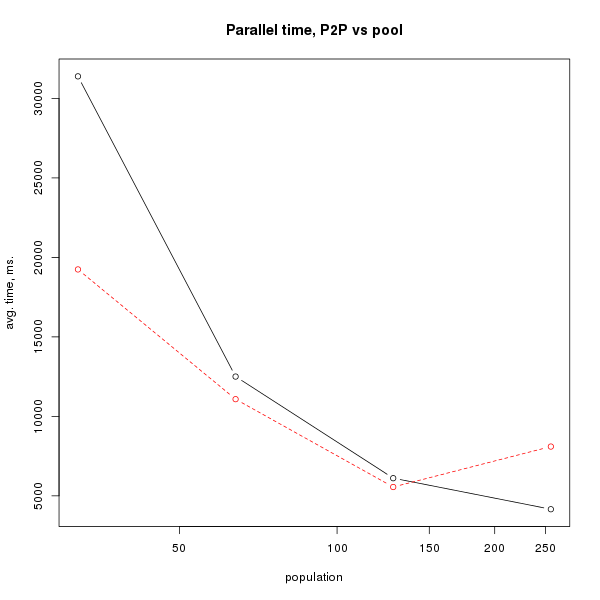
\includegraphics[scale=0.35]{par-pool-time-pop}
\caption{Average time, in milliseconds, for successful runs. Black,
  solid represents the previously mentioned P2P architecture, while
  the light, dashed line represents the pool-based, single-server
  architecture. }
\label{fig:p:time}
\end{figure}
%
\begin{figure}[htb]
\centering
   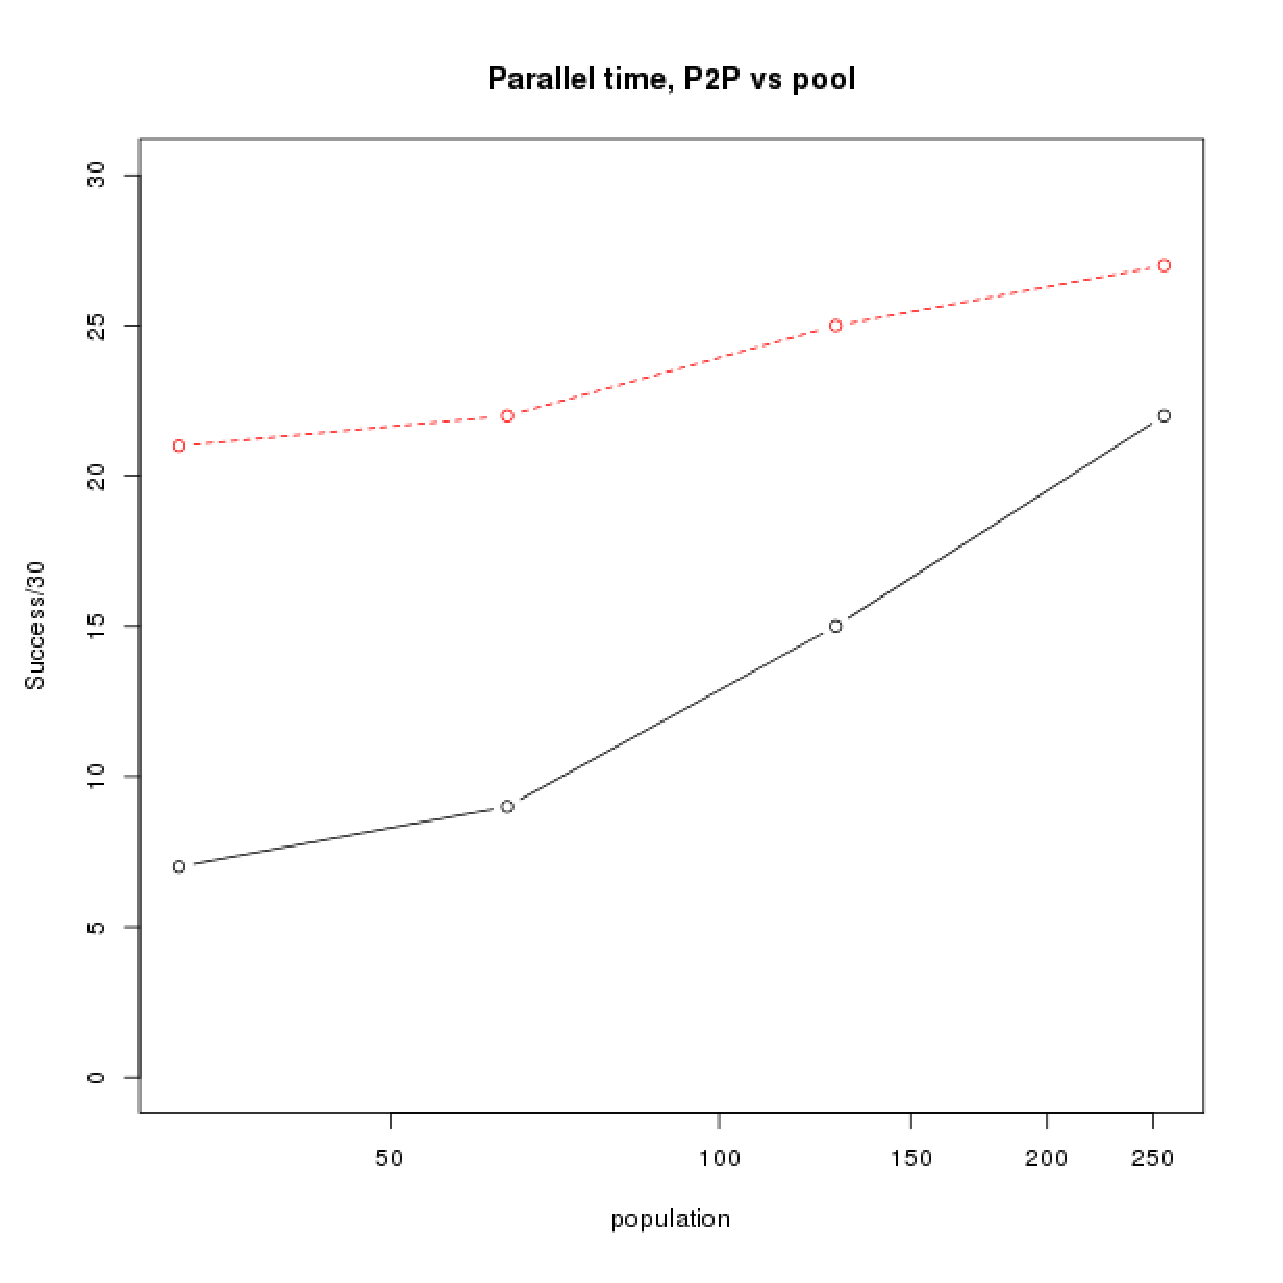
\includegraphics[scale=0.35]{par-pool-hits-pop}
\caption{Number of successful runs out of 30. Black, solid line
  corresponds to the P2P architecture, light-colored, dashed
corresponds to the single-server architecture (pool).}
\label{fig:p:hits}
\end{figure}
% Antonio - he puesto aqu� 'pool' porque las im�genes pueden salir lejos una de otra y as� son autocontenidas.


In general and from the point of view of the operating system load, no
great change is observed with the addition of one process ($n$ client
processes + server) to the pool; if there is any  difference in time, it
should not be attributed to increased OS load or, for that matter, to
the small changes in the application architecture done. Even if the
P2P applications do a single request (a GET) and this one performs two
(first a PUT and then a GET), it probably cancels out with the fact
that the P2P processes must also {\em respond} to requests from time
to time. In fact, what we observe in the comparison of both types of
architectures in Figure \ref{fig:p:time} is that there is a difference
for the smallest number of processes and the biggest number of
processes but they go in different directions, so it is difficult to
say if, in general, there is any difference (there is none for
$p=64,128$) and what is its origin. 

But a more dramatic change of scenario is shown in Figure
\ref{fig:p:hits}, which shows that the success rate is noticeably
higher for the pool-based architecture, although decreasingly so with the increasing population;
this is only to be expected since, in fact, success rate increased
with the population in the P2P architecture. This makes this pool-based
architecture from the
algorithmic point of view, the best alternative. Besides, they are not
mutually exclusive.

This conclusion is reached on top of having proved (yet again, some
might say) that JavaScript, its
implementation in {\tt node.js}, and the simple library called NodEO we are presenting in
this paper, are valid platforms for performing distributed computation
experiments, since they allow to create rapid prototypes to
concentrate on system architecture and the solution of problems via
evolutionary algorithms. In an unconstrained environment, JavaScript
will probably be slower than Java or C++, although its speed is on par with
other scripting languages like Ruby. However, in an environment
such as a multi-tier architecture that includes rich Internet
applications (with an UI written in JavaScript in the browser) or even
mobile applications (which can easily be done in JavaScript via the
PhoneGap framework or simply HTML5 in any browser) JavaScript can
offer an excellent performance and even algorithmic advantages in
distributed evolutionary algorithms, as  proved here.  

% Antonio - Creo hay que darle m�s bombo a esto porque el objetivo del trabajo parec�a ser que ofrec�a una alternativa MEJOR a lo que ya hay, es decir, mejor que las implementaciones de EAs en C y Java por ejemplo, pero eso no se comenta, s�lo se dice que JavaScript ofrece una implementaci�n V�LIDA... queda un poco flojo en ese sentido. :-(
% Pero es que no es mejor... simplemente otra alternativa. - JJ

\section{Conclusions}

In this paper we have proved the validity and performance {\tt node.js}-based distributed
evolutionary algorithm by using a standard module, NodEO. {\tt node.js} is better known in development and open source circles than in the scientific community, so our intention was to
introduce it to the evolutionary computation (EC) community by proving its
value as a platform for EC experiments. A basic EC library has been
created and released, so it is available to the researches. The
library can be expanded and, being open source, can be adapted and
suited to the needs of any particular user; due to the expansion of
the JavaScript and {\tt node.js} community, it should be increasingly easy
to find people interested and skilled enough to work in evolutionary
algorithms using JavaScript and {\tt node.js}, and, from the other end, it could get
the {\tt node.js} community interested in our area, which might prove the
source of interesting problems that can be dealt with from the point
of view of metaheuristics.


%ACKNOWLEDGMENTS are optionalndn
\section{Acknowledgments}

Funded by CEI-BioTIC grant CANUBE (CEI2013-P-14) and ANYSELF project (TIN2011-28627-C04-02). 

%
% The following two commands are all you need in the
% initial runs of your .tex file to
% produce the bibliography for the citations in your paper.
\bibliographystyle{abbrv}
\bibliography{geneura,javascript,ror-js}  % sigproc.bib is the name of the Bibliography in this case

\end{document}
